%!TeX root=../tese.tex
%("dica" para o editor de texto: este arquivo é parte de um documento maior)
% para saber mais: https://tex.stackexchange.com/q/78101

\chapter{Fundamentação teórica}

\section*{Aprendizado de máquina}

Atualmente, inteligência artificial (IA) permeia diversos momentos do cotidiano. É o caso da empresa norte-americana de \textit{streaming} Netflix, que utiliza um conjunto de técnicas de IA para recomendar conteúdo personalizado aos usuários da plataforma de acordo com os interesses particulares de cada um. Dessa forma, proporciona uma experiência única a cada indivíduo que acessa a plataforma com o objetivo de aumentar a satisfação a longo prazo e, consequentemente, garantir a retenção dos membros, uma vez que a plataforma é monetizada com assinaturas mensais. 

Além disso, não há um modelo ou algoritmo único utilizado para todas as recomendações de conteúdo. Essa tarefa é divida em subtarefas realizadas por diferentes modelos de acordo com a atividade a ser realizada e os dados disponíveis. Por exemplo, a subtarefa de  decidir qual vídeo será exibido para cada usuário ao logar no perfil da plataforma é executada por um modelo diferente do que o que elenca os vídeos já assistidos que o membro pode continuar a ver. \cite{netflix}

% pensar aqui se vale contar a historinha
% pode usar IBM ou precisa ser o nome completo?
Mas a final, o que é inteligência artificial (IA)? O termo "inteligência artificial", \textit{artificial intelligence} em inglês, foi elaborado por John McCarthy e utilizado oficialmente pela primeira vez em 1956 no seminário de Dartmouth, um \textit{workshop} sobre essa área que reuniu os maiores estudiosos do ramo durante dois meses. \cite{aima} Esse termo apresenta várias definições, de acordo com o pioneiro Arthur Samuel, pode ser definida como o campo de estudo que dá aos computadores a habilidade de aprender sem serem explicitamente programados. \cite{dl-oreilly} 

Aprendizado de máquina, por sua vez, do inglês \textit{machine learning}, são sistemas de IA capazes de adquirir seu próprio conhecimento por meio da extração de padrões dos dados brutos. Configura-se, portanto, como uma sub-área de inteligência artificial.\cite{Goodfellow-et-al-2016}. O aprendizado profundo, ou \textit{deep learning}, é uma categoria específica de \textit{machine learning} que compreende modelos de redes neurais com várias camadas de neurônios.\cite{d2l}

\begin{figure}[H] 
  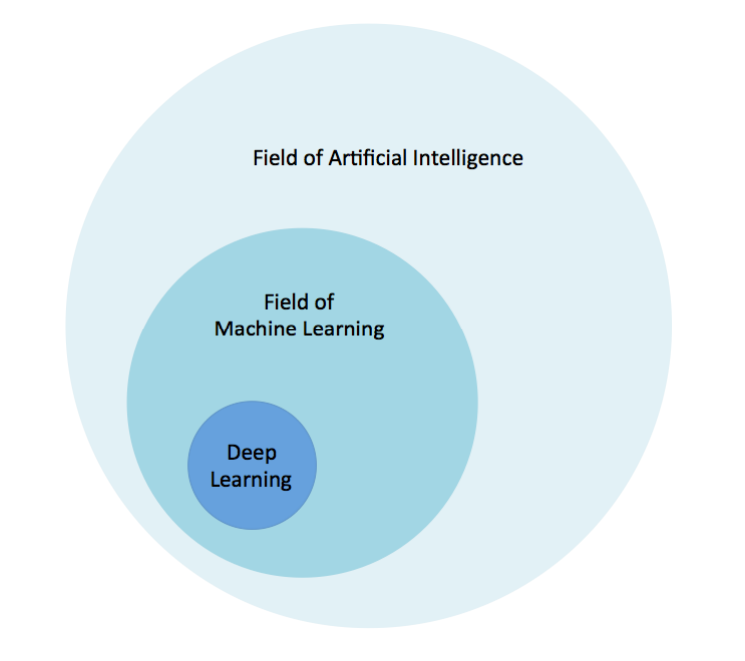
\includegraphics[width= 10cm]{../figuras/ia_ml.png}
  \caption{Relação entre inteligência artificial, aprendizado de máquina e aprendizado profundo \cite{dl-oreilly}}
\end{figure}

\section*{Problema}

As tarefas de \textit{machine learning} são descritas de acordo com o processamento que o modelo deve realizar a partir de um exemplo de entrada, em geral descrito com oum vetor $x \in \mathbb{R}^n$, por exemplo, neste trabalho um exemplo seriam os dados de março de 2011 do estado de São Paulo, cada entrada $x_i$, então corresponde à medição de um dos indicadores econômicos desse estado e tempo. Nas tarefas de classificação, o modelo deve prever a qual das $k$ categorias disponíveis um \textit{input} pertence. O algoritmo então cria uma função  $ f : \mathbb{R}^n \rightarrow {1,...,k}$,  quando $ f(x) = y$, o vetor de entrada $x$ foi recebeu a categoria $y$. Um exemplo de tarefa de classificação seria determinar se o consumo de cimento em um estado em um mês específico representa um aumento, queda ou estabilidade em relação ao mês anterior. Neste trabalho, contudo, não se utiliza essas tarefas.

Outra categoria de tarefas são as de regressão, aonde o objetivo é, a partir do \input{x}, prever um valor numérico. A função criada pelo modelo, então, é $ f : \mathbb{R}^n \rightarrow \mathbb{R}$. O problema abordado neste trabalho, então, configura-se como problema de regressão, uma vez que o objetivo é prever o valor do consumo de cimento em um estado e mês específicos a partir dos dados de entrada.

  %% Ver se não é melhor tirar pq opde ficar longo <---
  Os problemas de \textit{machine learning} pertencem a duas categorias principais: classificação ou regressão. As tarefas de classificação, por um lado, consistem em determinar a categoria, dentre as $k$ disponíveis, a que um \textit{input} pertence, um exemplo de tarefa de classificação seria determinar se o consumo de cimento em um estado em um mês específico representa um aumento, queda ou estabilidade em relação ao mês anterior. Os problemas de regressão, por outro lado, compreendem prever um valor numérico a partir de um \textit{input}, \cite{Goodfellow-et-al-2016} como adotado neste trabalho.

  
\section*{Regressão linear}
  % assume um relacionamento linear entre entrada e saída
  % dar uma melhorada na regressão
O modelo de regressão linear estabelece uma relação linear, ou seja, uma função, entre a variável que será prevista (\textit{target}) e as variáveis de entrada (\textit{predictor variables}), neste projeto: o consumo de cimento em um mês e estado determinados e os indicadores econômicos correspondentes, respectivamente. O algoritmo, então, calcula um coeficiente para cada \textit{predictor} afim de mensurar o efeito desse no \textit{target}, de modo a minimizar o erro na previsão.
     
\section*{Redes neurais}

\subsection*{Redes neurais multi-layer perceptrons}
  % dar uma melhorada -> parte do com o treinamento fornecido
  % se agredar -> combinação -> melhorar
  % redes de arquitetura multilayer ...
  % o "e feedforward" não tem nada a ver -> é um passo do treinamento  -> sequencia dos dados de entrada
Redes neurais são modelos de \textit{machine learning} inspiradas no cérebro humano aonde o aprendizado ocorre ao se agregarem neurônios matemáticos que estabelecem conexões de acordo com o treinamento fornecido. Neste trabalho, aplicaram-se redes \textit{multilayer perceptrons} (MLPs), ou seja, que apresentam múltiplas camadas de neurônios e \textit{feedfoward}, onde a saída de uma camada de neurônios é utilizada como entrada para a camada seguinte, sem utilizar retropropagação.
          
        
\subsection*{Redes Neurais Recorrentes}
  
Já as redes neurais recorrentes são projetadas para reconhecer padrões nos dados, uma vez que levam tempo e sequência em consideração. Assim, nessas redes, a decisão tomada na etapa anterior influencia a etapa seguinte por conta dos \textit{loops de feedback}, então o presente e o passado recente se combinam para determinar a previsão. Neste trabalho, foram testadas as redes Long Short Term Memory (LSTM), redes Gated Recurrent Unit (GRU) e Bidirecionais.
  
\subsubsection*{GRU}

\subsubsection*{LSTM}

\subsection*{Função de ativação}


\subsection*{Normalização}